\documentclass[9pt]{beamer}

% Use roboto Font (recommended)
\usepackage[sfdefault]{roboto}
%\usepackage[utf8]{inputenc}
%\usepackage[T1]{fontenc}

% Define where theme files are located. ('/styles')
\usepackage{flux-beamer/styles/fluxmacros}
\usefolder{flux-beamer/styles}
% Use Flux theme v0.1 beta
% Available style: asphalt, blue, red, green, gray 
\usetheme[style=asphalt]{flux}

% Extra packages for the demo:
\usepackage{booktabs}
\usepackage{colortbl}
\usepackage{ragged2e}
\usepackage{schemabloc}

\usepackage{xcolor}

\newcommand{\mascot}{../graphics/tux.png}

% Informations
\title{\#AdoptYourOwnPenguin}
\subtitle{Linux Install Party}
\author{Christoph Großmann \& Lea Laux}
\institute{Ministry of Silly Walks}
\date{\today}
\titlegraphic{\mascot}

\definecolor{background-local}{named}{background}
%\definecolor{Gray-local}{HTML}{858b8f}
%\definecolor{text-local}{HTML}{4F5D66}
%\definecolor{primaryLight-local}{HTML}{34495e}
%\definecolor{primary-local}{HTML}{2d3e50}
%\definecolor{secondary-local}{HTML}{d15306}
%\definecolor{tertiary-local}{HTML}{35837b}

\newcommand{\DarkBG}{\definecolor{background}{named}{primaryLight}}
\newcommand{\ResetBG}{\definecolor{background}{named}{background-local}}

\newcommand{\sectionframe}[1]{%
\DarkBG%
\begin{frame}[plain]%
\section{#1}\centering\Huge\color{background-local}\textbf{#1}%
\vfill\includegraphics[height=3cm]{\mascot}%
\end{frame}%
\ResetBG%
}

\begin{document}

	\titlepage
	
	\begin{frame}
	\frametitle{Table of contents}
	\tableofcontents
\end{frame}

	
	\sectionframe{Introduction to Linux}
	\begin{frame}
	\frametitle{Some information about Linux}
	\subsection{Some information}
	
	\vfill
	\begin{columns}
		\begin{column}{.7\linewidth}
			\begin{itemize}
				\item Operating systems based on the Linux kernel\cite{linux}
				\item The Linux kernel is part of the UNIX family
				\item (Mostly) open source
				\item Fit for a range of different use cases:
				\begin{tiny}
					\begin{itemize}
						\item Desctop computers
						\item Server
						\item Smartphones
						\item TVs
						\item Tablets
						\item IoT devices
						\item $\dots$
					\end{itemize}
				\end{tiny}
				\item Around since the mid-1990s
				\item Many of the supporting system software and libraries are provided by the GNU project\cite{gnu}
				\item Tux the penguin is the official mascot of Linux
			\end{itemize}
		\end{column}
		\hfill
		\begin{column}{.28\linewidth}
			\resizebox{\linewidth}{!}{\usebox\mascotbox}
		\end{column}
	\end{columns}
	\vfill
\end{frame}

	\begin{frame}
	\frametitle{Advantages of Linux}
	\subsection{Advantages of Linux}
	
	\begin{itemize}
		\item Open source
		\item Free
		\item A system under your exclusive control
		\item Multi-purpose
		\item Extremely costumisable
		\item Package managers
		\item $\dots$
	\end{itemize}

	\vfill
	
	There are some closed source programs. Most distributions give you the option whether to use them or not. Further there are some paid for Linux distributions but those are not particularly interesting for personal use.
\end{frame}

	\begin{frame}
	\frametitle{Linux distributions}
	\subsection{Linux distributions}
	
	\begin{columns}
		\begin{column}{.25\linewidth}
			Well known distros:
			\begin{itemize}
				\item Debian
				\item Ubuntu
				\item Arch Linux
				\item Manjaro
				\item openSuse
				\item Red Hat
				\item Fedora
				\item Kali
				\item Linux Mint
				\item $\dots$
			\end{itemize}
		\end{column}
		\hfill
		\begin{column}{.7\linewidth}
			\begin{figure}
				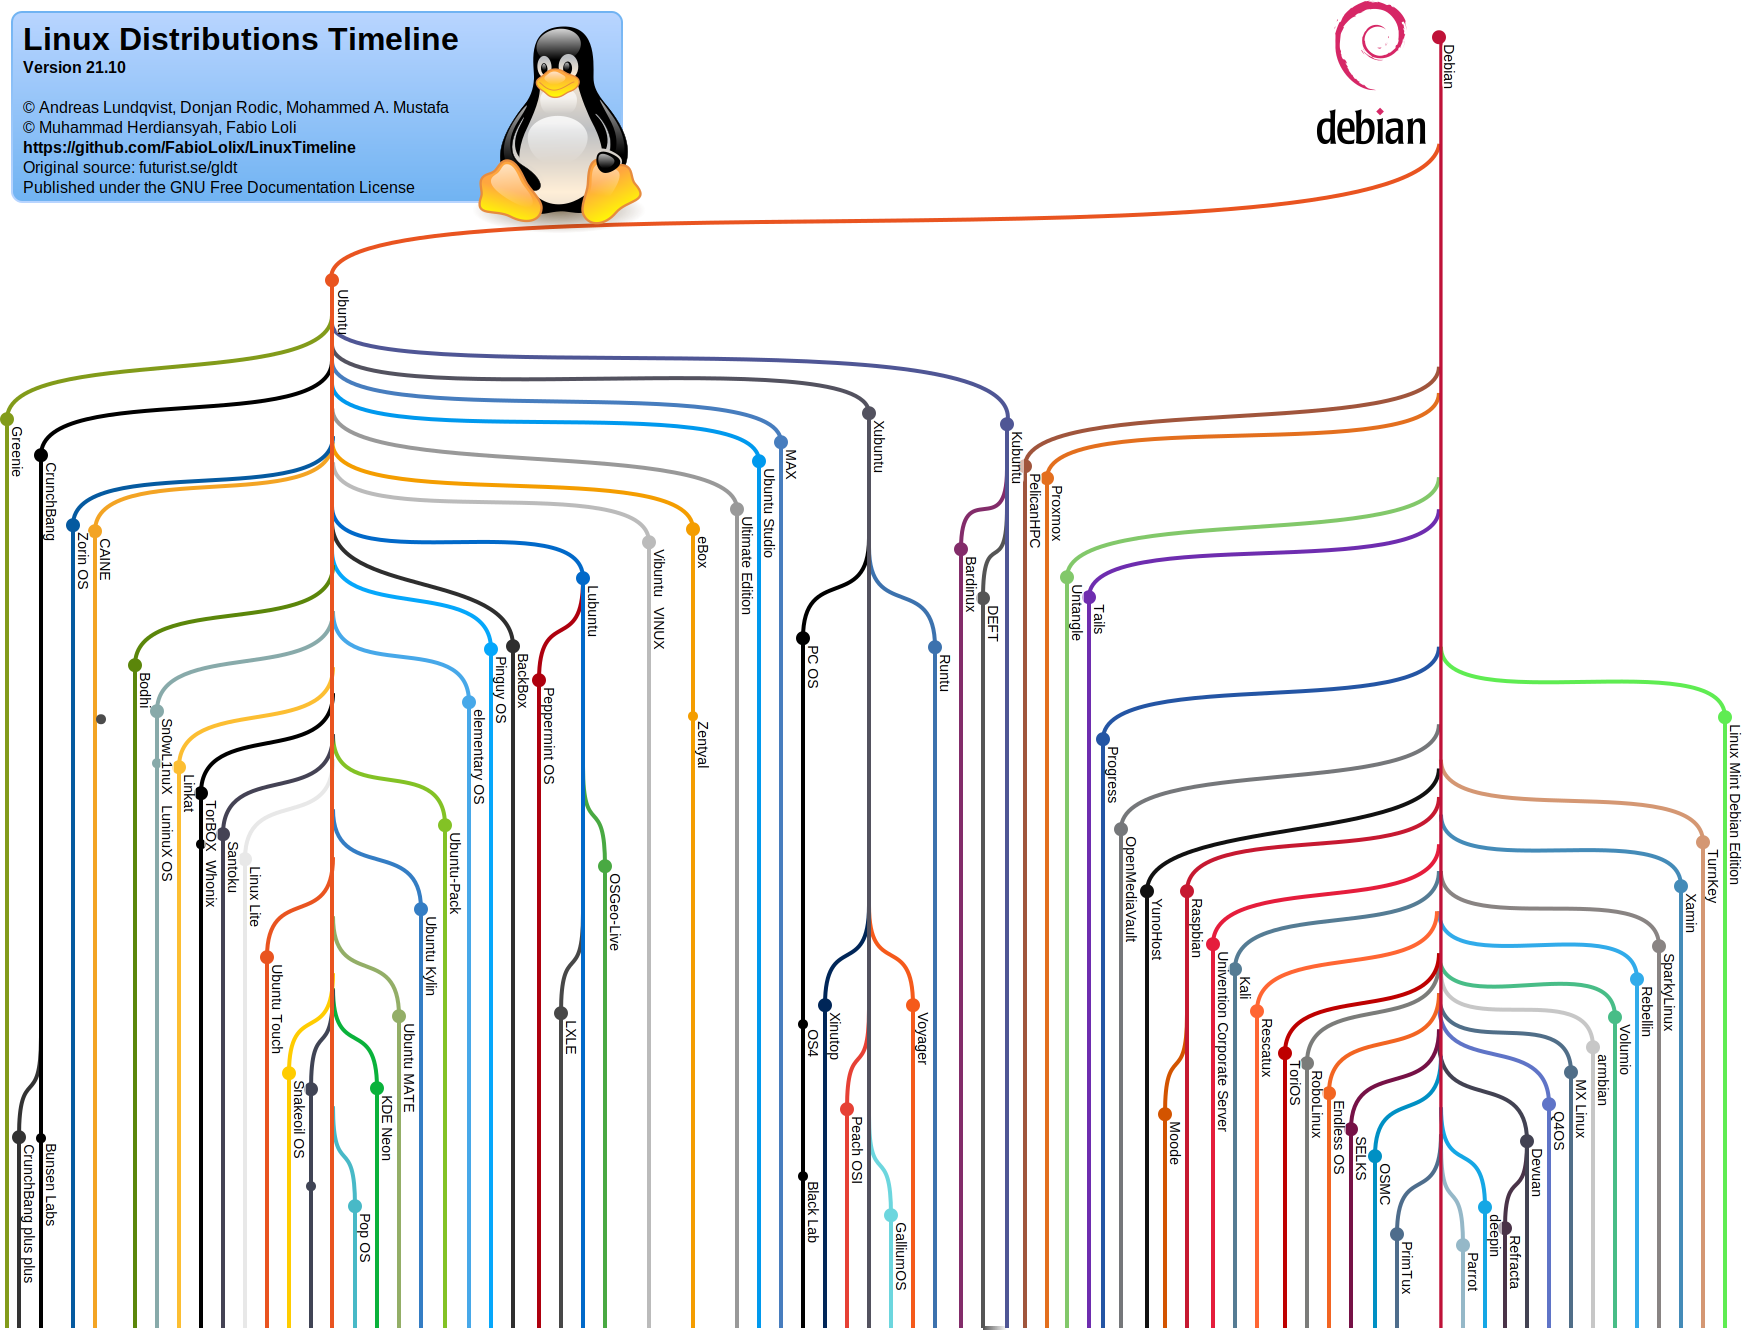
\includegraphics[width=\linewidth]{../graphics/debian_distro_timeline/debian_distro_timeline.png}
				\caption{Excerpt from the Linux distro tree for Debian \cite{distrograph}}
			\end{figure}
		\end{column}
	\end{columns}
	
	\vfill
	
	\centering
	See DistroWatch\cite{distrowatch} for a comprehensive list of all Linux distributions.
\end{frame}

	
	\sectionframe{A selection of noteworthy distributions}
	\begin{frame}
	\frametitle{Debian}
	\subsection{Debian}
	
	\vfill
	\begin{columns}
		\begin{column}{.65\linewidth}
			\begin{itemize}
				\item Around since 1993
				\item Comes with over 50,000 packages
				\item Supported desktop environments:
					\begin{tiny}
						\begin{itemize}
							\item XFCE
							\item GNOME
							\item KDE
							\item MATE
							\item Cinnamon
							\item LXDE
							\item MATE
						\end{itemize}
					\end{tiny}
				\item Release cycle
					\begin{itemize}
						\item A stable version is released every 2 years
						\item Each version will receive updates for 3 years
						\item Those updates will only contain security updates and fixes
						\item After that the version will receive security updates for 2 more years
						\item oldoldstable – oldstable – \textbf{stable} – testing
						– unstable – experimental
					\end{itemize}
				\item Package manager: \texttt{dpkg} / \texttt{apt}
			\end{itemize}
		\end{column}
		\hfill
		\begin{column}{.34\linewidth}
			\includegraphics[width=\linewidth]{../graphics/logos/Debian/openlogo.png}
		\end{column}
	\end{columns}
	\vfill
\end{frame}

	\begin{frame}
	\frametitle{Ubuntu and Linux Mint}
	\subsection{Ubuntu and Linux Mint}
	
	\begin{columns}
		\begin{column}[t]{.45\linewidth}
			\begin{block}{Ubuntu}
				\begin{itemize}
					\item Around since 2004
					\item Derivative of Debian
					\item Very new-user-friendly
					\item Default desktop: GNOME
					\item Packages are based on packages from Debian's unstable branch
					\item Release cycle
						\begin{itemize}
							\item New version every 6 months
							\item Long-term support version every 2 years
							\item LTS version updates for 5 years
						\end{itemize}
					\item Package manager: \texttt{apt}
				\end{itemize}
			\end{block}
		\end{column}
		\hfill
		\begin{column}[t]{.45\linewidth}
			\begin{block}{Linux Mint}
				\begin{itemize}
					\item Around since 2006
					\item Derivative of Ubuntu
					\item Also very new-user-friendly
					\item Default desktop: Cinnamon / MATE / Xfce
					\item Full out-of-the-box multimedia support
					\item Release cycle same as Ubuntu
					\item Package manager: \textit{dpkg} / \textit{Flatpak} / \texttt{apt}
				\end{itemize}
			\end{block}
		\end{column}
	\end{columns}
	
	\vfill
	
	\begin{columns}
		\begin{column}{.5\linewidth}
			\centering\includegraphics[height=3\baselineskip]{../graphics/logos/Ubuntu/ubuntu-logo-2022.png}
		\end{column}
		\hfill
		\begin{column}{.5\linewidth}
			\centering\includegraphics[height=3\baselineskip]{../graphics/logos/Mint/leaf.png}
		\end{column}
	\end{columns}
\end{frame}

	\begin{frame}
	\frametitle{Arch Linux and Manjaro}
	\subsection{Arch Linux and Manjaro}
	
	\begin{columns}
		\begin{column}[t]{.45\linewidth}
			\begin{block}{Arch Linux}
				\begin{itemize}
					\item Around since 2002
					\item Release cycle:
						\begin{itemize}
							\item Rolling release model
							\item Latest stable versions of most software
							\item \textbf{stable} – testing – unstable
							\item Quick access to new versions of software
						\end{itemize}
					\item Package manager: \texttt{pacman}
					\item Additional package repository called \textbf{A}rch \textbf{U}ser \textbf{R}epository
					\item Get the package manager \texttt{yay} if you can
					\item No visual installation!
				\end{itemize}
			\end{block}
		\end{column}
		\hfill
		\begin{column}[t]{.45\linewidth}
			\begin{block}{Manjaro}
				\begin{itemize}
					\item Around since 2011
					\item Derivative of Arch Linux
					\item Default desktop: Xfce / KDE Plasma / GNOME / Phosh
					\item Focus on user-friendliness and accessibility
					\item Still most of the benefits of Arch
					\item Visual installer
					\item Uses the same package repositories as Arch
					\item Package manager: \texttt{pacman}
				\end{itemize}
			\end{block}
		\end{column}
	\end{columns}
	
	\vfill
	
	\begin{columns}
		\begin{column}{.5\linewidth}
			\centering\includegraphics[height=3\baselineskip]{../graphics/logos/Arch/archlinux-logo-dark-1200dpi.b42bd35d5916.png}
		\end{column}
		\hfill
		\begin{column}{.5\linewidth}
			\centering\includegraphics[height=2\baselineskip]{../graphics/logos/Manjaro/Main_page_logo.png}
		\end{column}
	\end{columns}
\end{frame}

	\begin{frame}
	\frametitle{Linux Mint}
	\subsection{Linux Mint}
	
	bla, bla, bla, ...
\end{frame}

	
	\sectionframe{How to adopt a penguin}
	\begin{frame}
	\frametitle{Some information about Linux}
	\subsection{Some information}
	
	\vfill
	\begin{columns}
		\begin{column}{.7\linewidth}
			\begin{itemize}
				\item Operating systems based on the Linux kernel\cite{linux}
				\item The Linux kernel is part of the UNIX family
				\item (Mostly) open source
				\item Fit for a range of different use cases:
				\begin{tiny}
					\begin{itemize}
						\item Desctop computers
						\item Server
						\item Smartphones
						\item TVs
						\item Tablets
						\item IoT devices
						\item $\dots$
					\end{itemize}
				\end{tiny}
				\item Around since the mid-1990s
				\item Many of the supporting system software and libraries are provided by the GNU project\cite{gnu}
				\item Tux the penguin is the official mascot of Linux
			\end{itemize}
		\end{column}
		\hfill
		\begin{column}{.28\linewidth}
			\resizebox{\linewidth}{!}{\usebox\mascotbox}
		\end{column}
	\end{columns}
	\vfill
\end{frame}

	\begin{frame}
	\frametitle{Installing Linux}
	\subsection{Installing Linux}
	
	\begin{enumerate}
		\item Choose the distro you want to install.
		\item Make sure your machine meets the requirements for installation.
		\item Download the .iso-file you want.
		\item Write the .iso-file to USB-stick.
		\item Start your computer an enter the boot loader menu.
		\item Boot using the USB-stick as boot medium.
		\item Go through all installer steps and wait for the installation to finish.
	\end{enumerate}

	\vspace{\baselineskip}

	Well done, you've got yourself a Linux!
\end{frame}

	
	\sectionframe{How to handle a penguin}
	\begin{frame}
	\frametitle{Installing and updating software}
	\subsection{Installing and updating software}
	
	\begin{columns}
		\begin{column}{.45\linewidth}
			\begin{block}{Debian/Ubuntu/Mint}
				\begin{itemize}
					\item Get all new updates \bash{apt update}
					\item Install the updates \bash{apt upgrade}
					\item Install a package \bash{apt install [package]}
					\item Remove a package \bash{apt remove [package]}
					\item Search for a package \bash{apt search [package]}
				\end{itemize}
			\end{block}
		\end{column}
		\hfill
		\begin{column}{.45\linewidth}
			\begin{block}{Arch/Manjaro}
				\begin{itemize}
					\item Get and install all updates \bash{pacman -Syu}
					\item Install a package \bash{pacman -S [package]}
					\item Remove a package \bash{pacman -R [package]}
					\item Search for a package \bash{pacman -Ss [package]}
					\item Clean cache files \bash{pacman -Scc}
				\end{itemize}
			\end{block}
		\end{column}
	\end{columns}
\end{frame}

	\begin{frame}
	\frametitle{Troubleshooting}
	\subsection{Troubleshooting}
	
	bla, bla, bla, ...
\end{frame}

	
	%\begin{frame}%[allowframebreaks]{References}
	\frametitle{List of figures}
	
	\listoffigures
\end{frame}

	\begin{frame}%[allowframebreaks]{References}
	\frametitle{References}
	\section{References}
	
	\nocite{*}
	\bibliography{adoptyourownpenguin_presentation.bib}
	\bibliographystyle{abbrv}
\end{frame}

	\begin{frame}
	\frametitle{Flux beamer theme}
	
	Flux is a modern style beamer presentation. It is provided as a work in progress version and may suffer from inconsistencies. Sources and complementary information are available at:\\[.2\baselineskip]
	\url{github.com/pvanberg/flux-beamer}\\
	
	\vfill
	
	Flux is licensed under GNU General Public License v3.\\[.2\baselineskip]
	\url{http://www.gnu.org/licenses}\\
	
	\vfill
	
	Flux is inspired by \textbf{Metropolis} theme from Matthias Vogelgesang:\\[.2\baselineskip]
	\url{https://github.com/matze/mtheme} 
	
\end{frame}

	\begin{frame}
	\frametitle{This presentation}
	
	This presentation draws inspiration from presentation by Lea Laux, which you can find here:\\[.2\baselineskip]
	\url{https://github.com/LeaRain/LinuxInstallParty}
	
	\vfill
	
	This exact presentation can be found here:\\[.2\baselineskip]	
	\url{https://github.com/christoph-grossmann/AdoptYourOwnPenguin}
	
\end{frame}

	
	\DarkBG
\begin{frame}[plain]%
	\begin{columns}
		\hfill
		\begin{column}{.4\linewidth}
			\Huge\color{background-local}\textbf{Have fun with your new penguin!}
		\end{column}
		\hfill
		\begin{column}{.4\linewidth}
			\resizebox{\linewidth}{!}{\usebox\mascotbox}
		\end{column}
		\hfill
	\end{columns}
\end{frame}%
\ResetBG%


\end{document}
